\documentclass[a4paper,12pt]{article}

\usepackage[utf8]{inputenc}
\usepackage{polski}
\usepackage[polish]{babel}
\usepackage{graphicx}
\usepackage{url}
\usepackage{amsfonts}
\usepackage{amsmath}

\providecommand{\imref}[1]{Rys. \ref{#1}} % referencja do obrazka

%% Define a new 'leo' style for the package that will use a smaller font.
\makeatletter
\def\url@leostyle{%
  \@ifundefined{selectfont}{\def\UrlFont{\sf}}{\def\UrlFont{\small\ttfamily}}}
\makeatother
%% Now actually use the newly defined style.
\urlstyle{leo}

\begin{document}

\author{Jakub Kuźma}
\title{Pioneers - internetowa implementacja gry ,,Osadnicy z Catanu''
  w oparciu o framework Ruby on Rails}
\date{\today}

\begin{titlepage}
\maketitle
\end{titlepage}

\section{Analiza zagadnienia}

\subsection{Osadnicy z Catanu}
Gra planszowa ,,Osadnicy z Catanu'' została stworzona przez
niemieckiego matematyka Klausa Teubera. Po raz pierwszy została ona
wydana w 1995 roku w Niemczech pod nazwą \emph{Die Siedler von
  Catan}. O ogromnej popularności gry na całym świecie może świadczyć
fakt, iż została ona przetłumaczona na ponad 20 języków, w tym język
polski. Na całym świecie organizowane są turnieje gry, a począwszy od
roku 2000 organizowane są coroczne mistrzostwa świata. Pierwsze
polskie wydanie gry przypada na rok 2005. Od tego czasu organizowane
są corocznie Oficjalne Mistrzostwa Polski w ,,Osadników z Catanu'',
które w 2009 roku odbędą się w Gliwicach.

\subsection{Elementy gry}
Pierwotna wersja gry jest przeznaczona dla 3-4 graczy. Słowo pierwotna
jest tutaj szczególnie warte podkreślenia, gdyż ze względu na swą
ogromną popularność, gra doczekała się bardzo dużej ilości dodatków i
modyfikacji zasad. W tym podrozdziale postaram się omówić wszystkie
elementy wchodzące w skład gry. Moim celem nie jest omawianie zasad
gry, a jedynie ukazanie najważniejszych jej aspektów, które musiały
zostać uwzględnione przy implementacji.

\subsubsection{Plansza}
Rozgrywka toczy się na planszy złożonej z 37 sześciokątów
oznaczających różne rodzaje terenu oraz przypisanych do nich wartości
liczbowych. Poszczególne rodzaje pól mogą mieć także określony rodzaj
surowca, który może być z nich czerpany:

\begin{itemize}
\item las - drewno
\item pastwisko - wełna
\item pole uprawne - zboże
\item wzgórze - glina
\item góry - ruda żelaza
\item pustynia - brak surowca (początkowe położenie rozbójnika)
\item morze - brak surowca (może posiadać szlak handlowy)
\end{itemize}

Elementami planszy są również krawędzie i wierzchołki połączonych
sześciokątów. Na wierzchołkach (skrzyżowaniach) gracze mogą budować
osady i miasta. Przynoszą one dochód w postaci surowców z
sąsiadujących z nimi sześciokątów. Krawędzie natomiast przeznaczone są
pod budowę dróg, które łączą osady i miasta. Drogi nie przynoszą
żadnych dochodów, umożliwiają natomiast ekspansję terytorialną
(budowanie nowych osad).

Wszystkie surowce znajdujące się w posiadaniu poszczególnych graczy są
zakryte dla pozostałych uczestników gry. Zapamiętywanie surowców
otrzymanych przez pozostałych graczy jest bardzo istotnym elementem,
mającym duży wpływ na obraną strategię (m.in. na handel).

\subsubsection{Element losowy - kości do gry}
Gra ,,Osadnicy z Catanu'' jest grą umysłowo-losową. Głównym elementem
wprowadzającym do gry losowość, są dwie sześciościenne kości do
gry. Dla sumy dwóch rzutów kością prawdopodobieństwo uzyskania
poszczególnych wyników jest różne (zostało to przedstawione na
\imref{dice}). Sześciokąty na planszy (lasy, pastwiska, pola uprawne,
wzgórza i góry) mają przypisane wartości z przedziału 2-12, z
pominięciem liczby 7. Wszyscy gracze przed rozpoczęciem swojej tury
wykonują rzut kośćmi. Wynik rzutu oznacza, które sześciokąty przynoszą
w tej turze dochód. Surowce otrzymują tylko ci gracze, którzy są
posiadaczami osady lub miasta, które sąsiaduje z wylosowanym
sześciokątem. Przypisana wartość i rodzaj pola mają bezpośredni wpływ
na jego ,,atrakcyjność'' i co za tym idzie - na wybór strategii w
grze.

\begin{figure}[ht]
  \begin{center}
    \includegraphics[width=\linewidth]{dice.pdf}
  \end{center}
  \caption{Prawdopodobieństwa uzyskania poszczególnych wyników dla
    rzutu dwiema szcześciościennymi kośćmi do gry}
  \label{dice}
\end{figure}

\subsubsection{Karty rozwoju}
Kolejnym czynnikiem wprowadzającym w niewielkim stopniu losowość są
karty rozwoju. Za określoną ilość kart surowców gracz może nabyć kartę
rozwoju, ciągnąc ją z wierzchu potasowanego i zakrytego stosu. W grze
występuje pięć rodzajów kart:

\begin{itemize}
\item karta rycerza
\item karty postępu (,,monopol'', ,,budowa dróg'' i ,,wynalazek'')
\item karta ,,punkt zwycięstwa''
\end{itemize}

Karta rycerza stanowi element walki, element ten zostanie omówiony
później. Karty postępu w różny sposób przyspieszają rozwój
gracza. Ciekawym elementem jest jednak karta ,,punkt zwycięstwa'',
która stanowi istotny element zaskoczenia w grze. W związku z tym, że
po ,,zakupie'' karty rozwoju, jest ona zakryta dla pozostałych graczy,
nie znają oni rodzaju karty dopóki ta nie zostanie zagrana. Karty
,,punkt zwycięstwa'' ujawniane są bezpośrednio przed końcem gry. W
rezultacie gracz posiadający np. trzy karty rozwoju, może potencjalnie
posiadać trzy dodatkowe punkty zwycięstwa, które umożliwią mu znacznie
szybsze zakończenie gry.

\subsubsection{Handel}
Podczas rozgrywki gracze mają możliwość wymiany posiadanych surowców z
innymi graczami lub z bankiem.

Handel z bankiem odbywa się po określonych ,,kursach
wymiany''. Początkowo niekorzystne kursy można zmieniać poprzez
budowanie portów (osad) przy szlakach handlowych. Pozwalają one nawet
na dwukrotne zwiększenie korzystności takich wymian.

Przy handlu z innymi uczestnikami nie ma żadnych narzuconych z góry
,,kursów wymiany'' (zależą one wyłącznie od graczy). Zawsze jednak
musi to być wymiana - zabronione jest pozbywanie się surowców.

\subsubsection{Walka}
Ostatnim istotnym elementem gry jest ,,walka''. Zagranie karty armii
oraz wyrzucenie siódemki daje możliwość przesunięcia pionka,
tzw. ,,rozbójnika''. Pole zajmowane przez rozbójnika nie przynosi
graczom żadnego dochodu. Dodatkowo, po przesunięciu pionka, gracz ma
możliwość ,,obrabowania'' jednej z sąsiadujących z nim osad lub miast,
zabierając losowo wybraną kartę surowca od ich właściciela.

\subsubsection{Cel gry}
Celem gry jest zdobycie 10 punktów zwycięstwa, które są przyznawane
za:

\begin{itemize}
\item osadę - 1 punkt
\item miasto - 2 punkty
\item najdłuższą drogę - 2 punkty
\item największą armię - 2 punkty
\item kartę rozwoju ,,punkt zwycięstwa'' - 1 punkt
\end{itemize}

\clearpage

\section{Analiza istniejących rozwiązań}
W tym rozdziale przedstawiłem kilka powszechnie dostępnych,
działających rozwiązań. Wszystkie przedstawione implementacje gry
wymagają od użytkownika posiadania jakiegoś dodatkowego oprogramowania
(poza przeglądarką internetową). Większość z nich jest przystosowana
do jednej konkretnej platformy (np. PC z systemem Microsoft
Windows). Wadą tego typu rozwiązań jest to, że stworzenie wersji na
inną platformę (np. urządzenia mobilne) często wiąże się z
koniecznością stworzenia zupełnie nowej aplikacji.

\subsection{Pioneers}
Pierwotna nazwa tej aplikacji brzmiała \emph{gnocatan}. Aplikacja
została udostępniona w 2000 roku na licencji GNU GPL. Gra została
napisana całości w języku \emph{C}, podzielona jest na serwer i część
kliencką. Na stronie projektu \cite{pioneers} możemy znaleźć kod
źródłowy i wersje binarne, skompilowane na wszystkie popularne
platformy sprzętowe. Zrzut ekranu z gry \emph{Pioneers} został
przedstawiony na \imref{pioneers}.

\begin{figure}[ht]
  \begin{center}
    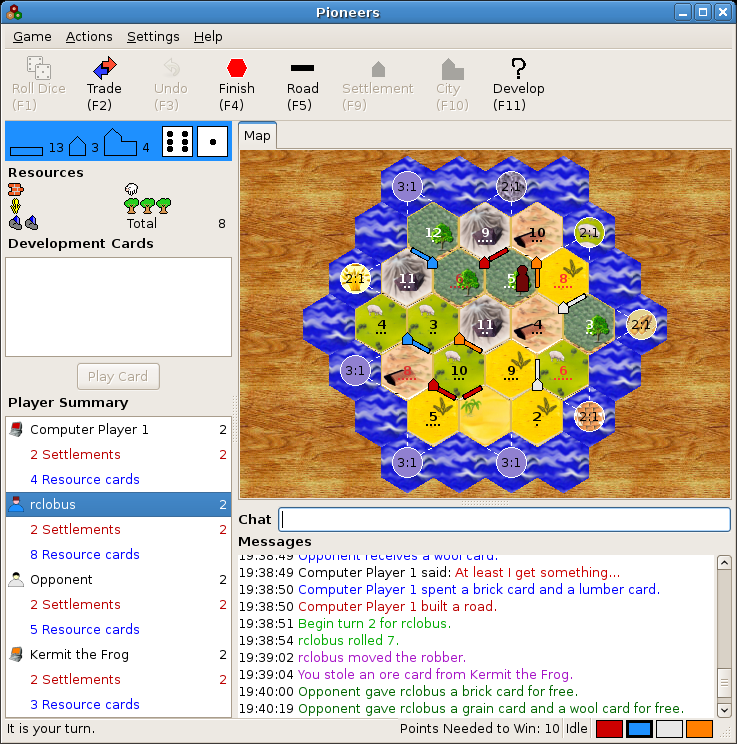
\includegraphics[width=\linewidth]{pioneers.png}
  \end{center}
  \caption{Zrzut ekranu z gry Pioneers}
  \label{pioneers}
\end{figure}

\subsection{JSettlers}
Aplikacja napisana w całości w Javie, rozwijana od początku 2004 roku
\cite{jsettlers}, dostępna na licencji GNU GPL. Aplikacja
przystosowana do uruchamiania w przeglądarce internetowej z
zainstalowanym środowiskiem uruchomieniowym Javy (\emph{ang. Java Runtime
  Environment}). Na \imref{jsettlers} został przedstawiony zrzut
ekranu z gry \emph{JSettlers}.

\begin{figure}[ht]
  \begin{center}
    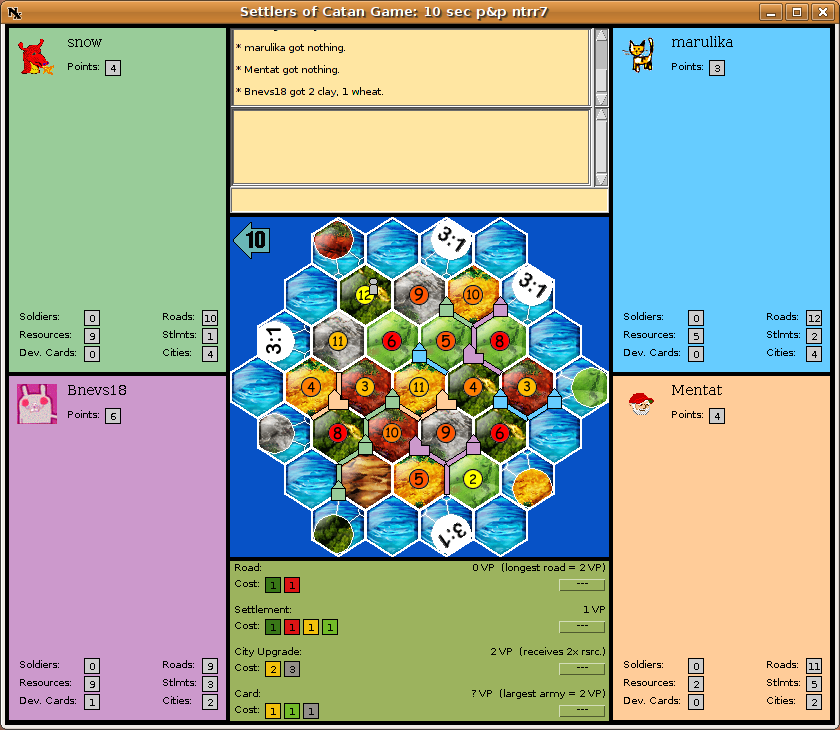
\includegraphics[width=\linewidth]{jsettlers.png}
  \end{center}
  \caption{Zrzut ekranu z gry JSettlers}
  \label{jsettlers}
\end{figure}

\subsection{Solito Server, MSN Games, PlayCatan.com}
Wszystkie te rozwiązania są oprogramowaniem własnościowym, w przypadku
dwóch ostatnich tytułów, płatnym. \emph{Solito Server} napisany został
przy użyciu technologii \emph{Adobe Flash}, dlatego jest w pewnym
stopniu uniezależniony od platformy sprzętowej (można go używać na
wszystkich platformach, na których dostępny jest \emph{Adobe
  Flash}). Pozostałe tytuły to oprogramowanie działające wyłącznie pod
kontrolą systemu operacyjnego \emph{Microsoft Windows}, wymagające
dodatkowo instalacji.

\subsection{Catan - The First Island}
Jest to prawdopodobnie jedyna implementacja gry dedykowana urządzeniom
mobilnym. Pierwotnie aplikacja napisana została w Javie dla urządzeń
mobilnych, przez niemiecką firmę \emph{Exozet Games}. W połowie 2009
roku pojawiła się także wersja przeznaczona dla konsoli \emph{Nintendo
  DS}. Oba rozwiązania umożliwiają rozgrywkę z graczem komputerowym
(\emph{AI}) oraz z innymi graczami poprzez \emph{Bluetooth} lub
\emph{WiFi}. Nie posiadają one niestety żadnego centralnego
serwera. Obie opisywane wersje są płatnym oprogramowaniem
własnościowym.

\clearpage

\section{Określenie funkcji aplikacji i wybór technologii}
Projektowana aplikacja składać się będzie z dwóch części: serwera i
klienta. Aplikacja w założeniu będzie wymagać bardzo dużego nakładu
pracy, w tym zaprojektowania interfejsu graficznego i stworzenia
grafiki. Aby umożliwić rozwój aplikacji, zdecydowałem się udostępnić
całość kodu jako wolne oprogramowanie na zasadach Powszechnej Licencji
Publicznej GNU Affero w wersji 3\cite{affero}.

Do zaimplementowania części serwerowej aplikacji zostanie wykorzystany
język \emph{Ruby} i framework \emph{Ruby on Rails}. Wybór można
uzasadnić bardzo dobrym wsparciem frameworka dla architektury
\emph{REST}, która zostanie wykorzystana do stworzenia \emph{API}.

\subsection{Ruby}
Język \emph{Ruby} został stworzony w 1995 roku przez Yukihiro
Matsumoto. Za bazę do jego stworzenia posłużyły języki takie jak
\emph{Lisp}, \emph{Perl}, \emph{Python}, \emph{Smalltalk}, a także
\emph{CLU} i \emph{Eiffel}. Jest to wieloparadygmatowy, dynamicznie
typowany, interpretowany język programowania bardzo wysokiego poziomu
(ang. \emph{VHLL} \footnote{VHLL - very high-level programming language
  \cite{vhll} }) \cite{ruby}. Najważniejszymi cechami języka są:

\begin{itemize}
\item pełna obiektowość - nie ma podziału na typy proste (wbudowane) i
  złożone. Pełnoprawnymi obiektami są także klasy, metody, wyrażenia
  lambda, itp.
\item pseudoklasyczny mechanizm dziedziczenia jednobazowego
\item moduły oferujące mechanizm zastępujący dziedziczenie wielobazowe
  (ang. \emph{mixin} \cite{mixin})
\item otwarte klasy, pozwalające na zmianę w dowolnym momencie
  wykonywania programu właściwości zdefiniowanych już klas (włącznie z
  klasami pochodzącymi z biblioteki standardowej języka)
\item \emph{monkey patching} - wykorzystanie mechanizmu otwartych klas
  do zmiany działania już istniejącego kodu w czasie wykonywania
  programu \cite{monkeypatch}
\item metaprogramowanie - mechanizm ten umożliwia tworzenie kodu,
  który generuje kod w czasie wykonywania programu
  \cite{metaprogramming}
\item ,,kacze typowanie'' - typy obiektów przekazywanych jako
  argumenty funkcji nie są w żaden sposób sprawdzane. Dzięki temu nie
  jest konieczne tworzenie skomplikowanych hierarchii dziedziczenia
  klas, wystarczy jedynie zaimplementować w klasach pewien wspólny
  podzbiór właściwości wymaganych przez wywoływaną na nich funkcję
  \cite{ducktyping}
\item domknięcia - mechanizm wiązania tworzonych funkcji z ich
  otoczeniem. Podczas wywołania funkcji ma ona dostęp do zmiennych,
  które zostały dowiązane do niej podczas jej tworzenia (nawet jeśli
  są one niedostępne podczas jej wywołania) \cite{closures}
\item przejrzysta, czytelna składnia
\item bogata biblioteka standardowa
\end{itemize}

Język \emph{Ruby} doczekał się wielu różnych implementacji, z których
najbardziej dojrzałe są:

\begin{itemize}
\item \emph{Matz's Ruby Interpreter} (\emph{MRI}) - intepreter
  stworzony w języku \emph{C}, uznawany \emph{de facto} za
  implementację referencyjną\cite{mri}
\item \emph{JRuby} - interpreter stworzony w języku Java,
  uruchamiany w \emph{wirtualnej maszynie Javy}\cite{jruby}
\end{itemize}

Głównym wskaźnikiem świadczącym o dojrzałości interpretera jest
możliwość uruchomienia na nim frameworka \emph{Ruby on
  Rails}. Wymienione wyżej implementacje najczęściej wykorzystywane są
do budowy środowisk produkcyjnych. Pozostałe implementacje są w
większości w fazie rozwoju, zaliczają się do nich
m.in. \emph{Cardinal}, \emph{IronRuby}, \emph{MacRuby}, \emph{MagLev},
\emph{Rubinius}, \emph{Ruby.NET} oraz \emph{XRuby}.

Ogromną zaletą języka \emph{Ruby} jest fakt, iż wszystkie wyżej
wymienione implementacje, za wyjątkiem \emph{MagLev}, to wolne
oprogramowanie. Rozwojem języka kieruje społeczność, tworząca kod
\emph{MRI}, nie jest on uzależniony od żadnych zewnętrznych firm (jak
ma to miejsce w przypadku języka \emph{Java} i firmy \emph{Sun
  Microsystems}).

W związku z tym, że język \emph{Ruby} utożsamiany jest głównie z
technologiami webowymi, należałoby nadmienić fakt, iż tworzenie
aplikacji internetowych nie miało wpływu na rozwój tego języka (tak
jak ma to miejsce w przypadku języka \emph{PHP}). Zamierzeniem
Yukihiro Matsumoto było stworzenie języka, który byłby
,,skuteczniejszy niż \emph{Perl} oraz bardziej zorientowany obiektowo
niż \emph{Python}''\cite{matzinterview}. Język \emph{Ruby} posiada
bardzo bogatą bibliotekę standardową, a także dużą ilość bibliotek
zewnętrznych (tzw. \emph{gemów}). Równie dobrze nadaje się do
tworzenia aplikacji okienkowych, serwerów sieciowych, jak i skryptów
systemowych. Nie zmienia to jednak faktu, że popularność języka wiąże
się nierozłącznie z frameworkiem \emph{Ruby on Rails}.

\subsection{Ruby on Rails}
Twórcą frameworka \emph{Ruby on Rails} jest duński programista David
Heinemeier Hansson. Framework powstał w wyniku prac nad aplikacją
\emph{Basecamp}, został udostępniony w połowie 2004 roku. Wzrost
popularności \emph{Ruby on Rails} nastąpił po ogłoszeniu przez firmę
\emph{Apple Inc.}, że będzie on dostarczany wraz z systemem \emph{Mac
  OS X v10.5 ''Leopard''}\cite{rubyonrails}. Swoje ogromne możliwości
framework zawdzięcza wykorzystaniu cech takich języka, jak:
metaprogramowanie, kacze typowanie czy możliwość otwierania klas.

Framework \emph{Ruby on Rails} umożliwia tworzenie aplikacji
internetowych w oparciu o wzorzec \emph{MVC}\footnote{MVC -
  model-widok-kontroler (ang. Model-View-Controller), wzorzec
  projektowy, którego założeniem jest podział aplikacji na modele,
  widoki i kontrolery. Podział jest realizowany w taki sposób, aby
  modyfikacja jednego elementu miała jak najmniejszy wpływ na
  działanie pozostałych\cite{mvc}}. \emph{Ruby on Rails} obsługuje
wszystkie popularne silniki bazodanowe poprzez bibliotekę mapowania
obiektowo-relacyjnego \emph{ActiveRecord} \cite{orm}. Aplikacje
napisane przy użyciu frameworka mogą być uruchamiane na serwerach
webowych, takich jak \emph{Apache}, \emph{Lighttpd}, \emph{Abyss},
\emph{Thin}, \emph{Mongrel}. W przypadku zastosowania \emph{JRuby},
mogą być to m.in. serwery aplikacji \emph{JBoss}, \emph{GlassFish} lub
\emph{Apache Geronimo}.

Cały framework jest udostępniony na zasadach licencji \emph{MIT}
\cite{mit}.

\subsubsection{Architektura Ruby on Rails}
Framework \emph{Ruby on Rails} składa się z komponentów, z których
główne to:

\begin{itemize}
\item \emph{ActiveRecord} - biblioteka mapowania
  obiektowo-relacyjnego, stworzona na podstawie wzorca projektowego o
  tej samej nazwie\cite{activerecord}. Biblioteka ta oferuje znacznie
  więcej, niż wynika z implementowanego wzorca, m.in. różne rodzaje
  asocjacji (w tym asocjacje polimorficzne\cite{polymorphic}),
  mechanizm dziedziczenia jednotabelowego (\emph{STI}\footnote{STI -
    dziedziczenie jednotabelowe (ang. Single Table Inheritance) -
    technika umożliwiająca odzwierciedlenie w jednej tabeli relacyjnej
    bazy danych obiektów wielu dziedziczących po sobie
    klas\cite{sti}}) oraz walidatory
\item \emph{ActionPack} - biblioteka umożliwiająca tworzenie
  kontrolerów i widoków, odpowiada również za kierowanie zapytań do
  odpowiednich akcji kontrolerów (tzw. \emph{routing})
\item \emph{ActiveSupport} - biblioteka dodająca wiele użytecznych
  funkcji do klas biblioteki standardowej, ułatwiających tworzenie
  aplikacji webowych (i nie tylko)
\item \emph{ActionMailer} - biblioteka służąca do wysyłania wiadomości
  e-mail, np. poprzez zewnętrzne serwery \emph{SMTP}
\item \emph{ActiveResource} - biblioteka umożliwiająca mapowanie
  zasobów \emph{REST}\footnote{REST - ang. Representational State
    Transfer, styl architektury zakładający traktowanie informacji
    udostępnianych przez aplikacje webowe jako zasoby, na których
    wywoływane są działania takie jak: tworzenie zasobu, odczyt,
    aktualizacja i usuwanie (ang. create, read, update,
    delete)\cite{rest}} na modele w aplikacji
\end{itemize}

Uproszczony diagram przedstawiający interakcje pomiędzy poszczególnymi
elementami frameworka został przedstawiony na
\imref{railsarchitecture}.

\begin{figure}[ht]
  \begin{center}
    \includegraphics[width=\linewidth]{railsarchitecture.png}
  \end{center}
  \caption{Architektura Ruby on Rails}
  \label{railsarchitecture}
\end{figure}

\subsubsection{Rozwój Ruby on Rails}
Na początku roku 2008 światło dzienne ujrzał nowy framework do
tworzenia aplikacji webowych o nazwie \emph{Merb}, silnie inspirowany
przez \emph{Ruby on Rails}. Został on stworzony z inicjatywy Ezry
Zygmuntowicza, założyciela firmy \emph{Engine Yard}. W założeniach
oprogramowanie miało być szybsze i bardziej modularne niż jego
pierwowzór. Spory pomiędzy zwolennikami nowopowstałego frameworka a
dotychczasową społecznością spowodowały powstanie w niej pewnego
rodzaju rozłamu. Przy narastającej fali krytyki z obu stron, niedługo
po wydaniu \emph{Merba 1.0}, David Heinemeier Hansson ogłosił
połączenie obu grup programistów\cite{merge}. Utworzony zespół miał
się zająć połączeniem powstającego \emph{Merba 2} i \emph{Ruby on
  Rails 3}. Zgodnie z ustaleniami, pierwsze wydania \emph{Ruby on
  Rails 3} mają się pojawić pod koniec 2009 roku.

\subsection{JavaScript}
Język \emph{JavaScript} powstał pod koniec 1995 roku w firmie
\emph{Netscape Communications Corporation}, jako alternatywa dla
uruchamianych w przeglądarce apletów \emph{Javy}. Jego twórcą jest
amerykański programista Brendan Eich. Począwszy od 1996 roku język
jest standaryzowany przez \emph{ECMA International}\footnote{ECMA -
  Europejskie Stowarzyszenie na rzecz Standaryzacji Systemów
  Informacyjnych i Komunikacyjnych (ang. European association for
  standardizing information and communication systems), organizacja
  zajmująca się standaryzacją systemów informatycznych w
  Europie\cite{ecma}} jako \emph{ECMAScript}.

Pomimo swojej nazwy jasno kojarzącej się z językiem \emph{Java}, język
\emph{JavaScript} jest (z wyjątkiem kilku elementów) językiem
diametralnie od \emph{Javy} różnym. Największy wpływ na jego rozwój
miały języki takie jak: \emph{Self}, \emph{C}, \emph{Scheme},
\emph{Perl} oraz \emph{Python}\cite{javascript}. Aby upodobnić język
do błyskawicznie zyskującej wówczas popularność \emph{Javy},
zapożyczony został zestaw słów kluczowych i składnia. Ta prosta
marketingowa sztuczka zaowocowała całkowitym niezrozumieniem tego
języka przez programistów, którzy przez wiele lat traktowali go jako
pewien podzbiór języka \emph{Java}. W rzeczywistości, język
\emph{JavaScript} jest znacznie bliżej spokrewniony z językami
funkcyjnymi, takimi jak \emph{Lisp}.

Interpreter \emph{JavaScriptu} wbudowany jest w niemal każdą
współczesną przeglądarkę internetową, co czyni go jednym z najbardziej
rozpowszechnionych języków programowania na świecie.

Najważniejszymi cechami języka, wyróżniającymi go od języków
,,c-pochodnych'' (w tym od \emph{Javy}) są:

\begin{itemize}
\item dynamiczne typowanie
\item domknięcia
\item prawie całkowita obiektowość - występuje podział na typy proste
  i obiekty. Obiekty są tablicami asocjacyjnymi, ich właściwości można
  dowolnie modyfikować podczas wykonania programu (w praktyce
  mechanizm ten jest bardzo podobny do ,,otwierania klas'' w języku
  \emph{Ruby}).
\item dziedziczenie prototypowe - mechanizm dziedziczenia
  bezklasowego. Jedyną cechą umożliwiającą stwierdzenie pokrewieństwa
  obiektów jest posiadanie przez nie wspólnego prototypu
\end{itemize}

Główne implementacje \emph{JavaScriptu} to\cite{javascript}:

\begin{itemize}
\item \emph{SpiderMonkey} - pierwszy interpreter, napisany przez
  twórcę języka w \emph{C}, wykorzystywany m.in. w przeglądarce \emph{Mozilla
    Firefox}.
\item \emph{Rhino} - interpreter napisany w \emph{Javie}, pozwala na
  uruchamianie \emph{JavaScriptu} na wirtualnej maszynie \emph{Javy}
\item \emph{KDE's JavaScript engine} - wykorzystywany w przeglądarce
  \emph{Konqueror}
\item \emph{WebKit} - napisany w \emph{C++} interpreter używany
  m.in. w przeglądarce \emph{Safari} firmy \emph{Apple Inc.}
\item \emph{V8} - zaimplementowany w \emph{C++} interpreter używany w
  przeglądarce \emph{Google Chrome}
\end{itemize}

Rozmaite dialekty \emph{JavaScriptu} (a dokładniej standardu
\emph{ECMAScript}) znalazły się także poza przeglądarkami
internetowymi. Wśród nich wyróżnić można m.in.:

\begin{itemize}
\item \emph{JScript} - dialekt stworzony i rozwijany przez firmę
  \emph{Microsoft}. Oprócz wbudowania w przeglądarkę \emph{Microsoft
    Internet Explorer} interpreter tego dialektu jest również częścią
  środowiska \emph{Microsoft Windows Scripting Host}, jest to także
  jeden z podstawowych języków środowiska \emph{.NET}
\item \emph{ActionScript} - dialekt rozwijany przez firmę \emph{Adobe
    Systems}, wykorzystywany w środowisku \emph{Adobe Flash}
\end{itemize}

\subsubsection{XMLHttpRequest (Ajax)}
Po rozpowszechnieniu się \emph{JavaScriptu} w przeglądarkach
internetowych, był on używany głównie do ,,upiększania'' stron
\emph{HTML} i dodawania do nich dynamicznych elementów. Stał się swego
rodzaju dodatkiem, ułatwiającym korzystanie ze stron.

Sytuacja zaczęła się zmieniać po wprowadzeniu przez firmę
\emph{Microsoft} obiektu \emph{ActiveX} nazwanego \emph{XMLHTTP} w
przeglądarce \emph{Microsoft Internet Explorer 5}. Najważniejszą cechą
tego mechanizmu była możliwość komunikacji z serwerem bez konieczności
przeładowywania całego dokumentu. W krótkim czasie podobne rozwiązania
zostały zaimplementowane w konkurencyjnych przeglądarkach, m.in.w
\emph{Mozilli} i \emph{Safari}. Pomimo tego, że funkcje te były
dostępne w przeglądarkach od końca 1999 roku, pierwsze duże aplikacje
zaczęły z nich korzystać dopiero w 2004 roku. Najważniejszymi
aplikacjami, które spopularyzowały opisywany mechanizm były
\emph{Gmail} i \emph{Google Maps}, stworzone przez firmę \emph{Google
  Inc.} W 2005 roku wprowadzony został termin \emph{Ajax}
(ang. asynchronous JavaScript and XML), oznaczający wykorzystanie
języków \emph{JavaScript} i \emph{XML} do asynchronicznej komunikacji
z serwerem\footnote{w rzeczywistości jednak, żaden z wymienionych
  elementów nie jest wymagany. W niektórych przeglądarkach zamiast
  \emph{JavaScriptu} można użyć innego języka (np. \emph{VBScript}),
  zamiast \emph{XML}-a często jest używany \emph{JSON} lub zwykły
  tekst, a zapytania wcale nie muszą być asynchroniczne\cite{ajax}}.

W związku z ograniczeniami narzucanymi przez przeglądarki internetowe,
wszystkie zapytania wykonywane przy pomocy skryptów muszą odwoływać
się do domeny, z której pobrany został dokument \emph{HTML} (ang. same
origin policy\cite{origin}). Dla aplikacji wymagających komunikacji z
różnymi domenami (np. ściągającymi dane z innych aplikacji) powstało
rozwiązanie nazwane \emph{JSONP}. W uproszczeniu polega ono na
dodawaniu do kodu dokumentu \emph{HTML} tagu \texttt{<script>}. Tag
ten może zostać dodany z wnętrza działającego w przeglądarce skryptu,
spowoduje on załadowanie i zinterpretowanie przez przeglądarkę kodu
pochodzącego z dowolnej domeny\cite{json}. Rozwiązanie to jest używane
do przesyłania danych w formacie \emph{JSON}. Przesyłany obiekt musi
być otoczony wywołaniem funkcji zwrotnej (ang. callback), w celu
poinformowania skryptu o otrzymaniu danych. Podobne rozwiązanie jest
używane również do tzw. leniwego ładowania kodu aplikacji (dynamiczne
ładowanie zależności). Należy zaznaczyć, że ładowanie kodu z innych
domen jest potencjalnie niebezpiecznym działaniem i powinno być
wykorzystywane z dużą rozwagą.

\subsubsection{HTTP Push (Comet)}
W przypadku standardowego wykorzystania technologii \emph{Ajax},
przesyłanie danych odbywa się na żądanie przeglądarki internetowej. W
niektórych rozwiązaniach taki mechanizm jest zbyt mało wydajny i
wprowadza w komunikacji niepożądane opóźnienia. Najprostszym
przykładem takiej aplikacji jest czat. W klasycznym rozwiązaniu każdy
klient musi co pewien czas odpytywać serwer o to, czy pojawiły się na
nim jakieś nowe wiadomości. Im mniejszy jest czas pomiędzy
poszczególnymi zapytaniami, tym większa jest ilość wykonywanych
zapytań i co za tym idzie, tym większe jest obciążenie
serwera. Technika ta jest także nazywana \emph{HTTP
  Pull}\footnote{ang. pull technology, client pull - styl komunikacji
  sieciowej, w którym wszystkie połączenia są inicjowane przez
  klienta\cite{pull}}, schemat jej działania został przedstawiony na
\imref{pull}.

\begin{figure}[ht]
  \begin{center}
    \includegraphics[width=\linewidth]{pull.pdf}
  \end{center}
  \caption{Schemat działania mechanizmu odpytywania (\emph{HTTP
      Pull})}
  \label{pull}
\end{figure}

Jeśli przyjrzeć się bliżej aplikacji takiej jak \emph{Gmail} okazuje
się, że nie wykonuje ona cyklicznego odpytywania serwera, a wszystkie
dane przesyłane są do klienta niemalże bez opóźnień. Najprostszym
sposobem na uniknięcie częstego odpytywania serwera jest zastosowanie
mechanizmu wydłużonego odpytywania (ang. long polling). Polega on na
wydłużaniu czasu trwania zapytań poprzez opóźnianie reakcji
serwera. Jeśli po otrzymaniu zapytania na serwerze nie ma żadnych
danych do pobrania, zamiast wysyłać informację o braku danych serwer
wstrzymuje się z odpowiedzią do czasu ich nadejścia. W przypadku, gdy
na serwerze pojawią się dane, są one natychmiast wysyłane do klienta
poprzez otwarte połączenie. W przypadku, gdy zostanie przekroczony
maksymalny czas trwania połączenia (ang. timeout) jest ono zamykane. W
obu przypadkach klient natychmiastowo wywołuje kolejne zapytanie,
które ponownie oczekuje na pojawienie się danych. Schemat działania
takiego mechanizmu został przedstawiony na \imref{longpolling}.

\begin{figure}[ht]
  \begin{center}
    \includegraphics[width=\linewidth]{longpolling.pdf}
  \end{center}
  \caption{Schemat działania mechanizmu wydłużonego odpytywania}
  \label{longpolling}
\end{figure}

Niewątpliwą wadą przedstawionego rozwiązania jest fakt, iż w
przypadku, gdy dane pojawiają się na serwerze z dużą częstotliwością,
wywoływanych jest dużo pojedynczych zapytań. Skutkuje to oczywiście
wzrostem obciążenia serwera. W mechanizmie wydłużonego odpytywania
wykorzystywane są asynchroniczne zapytania \emph{XMLHttpRequest}. W
przypadku pobierania danych z domen innych wykorzystywany jest
mechanizm \emph{JSONP}.

Innym, bardziej wyrafinowanym sposobem komunikacji poprzez \emph{HTTP
  Push} jest strumieniowanie danych. Do strumieniowania danych
wykorzystywany jest fakt, iż wszystkie współczesne przeglądarki
internetowe renderują strony progresywnie.
% potrzebne źródło
W związku z tym, możliwe staje się stworzenie ,,nieskończonego''
zapytania, które będzie interpretowane przez silnik na bieżąco, w
chwili pojawiania się nowych elementów. Do stworzenia takiego
zapytania wykorzystywany jest ukryty znacznik
\texttt{<iframe>}. Znacznik ten umożliwia zagnieżdżenie w dokumencie
innego dokumentu, pochodzącego z innego adresu
internetowego\footnote{w tym przypadku również nie jest możliwe
  załadowanie dokumentu z innej domeny, zgodnie z polityką
  bezpieczeństwa przeglądarek}. Podobnie jak w przypadku \emph{JSONP}
przesyłane dane muszą być otoczone wywołaniem funkcji, która ma je
odebrać. Dodatkowo całość musi zostać otoczona znacznikiem
\texttt{<script>}. Każdy taki znacznik jest renderowany
(interpretowany) przez przeglądarkę zaraz po jego otrzymaniu. W
przypadku, gdy na serwerze nie ma żadnych danych, wysyłany jest co
pewien czas pusty znacznik, w celu utrzymania połączenia. Schemat
działania mechanizmu strumieniowania został przedstawiony na
\imref{streaming}.

\begin{figure}[ht]
  \begin{center}
    \includegraphics[width=\linewidth]{streaming.pdf}
  \end{center}
  \caption{Schemat mechanizmu strumieniowania danych}
  \label{streaming}
\end{figure}

W związku z tym, że opisywane mechanizmy wykorzystują techniki
nieobjęte żadną specyfikacją, ich działanie jest w dużej mierze
zależne od implementacji poszczególnych przeglądarek
internetowych. Największym wyzwaniem jest przystosowanie wymienionych
technik do przeglądarek w urządzeniach mobilnych. Okazuje się również,
że użycie \emph{HTTP Push} na powszechnie używanych serwerach
\emph{HTTP} jest wysoce nieefektywne lub wręcz niemożliwe. Niemal
wszystkie dostępne rozwiązania wymagają uruchomienia dodatkowych
serwerów, odpowiedzialnych wyłącznie za obsługę \emph{HTTP Push}. Są
to serwery takie jak: \emph{Caplin Liberator}, \emph{Cometd},
\emph{ErlyComet}, \emph{GlassFish}, \emph{Jetty},
\emph{Lightstreamer}, \emph{Meteor}, \emph{Orbited}, \emph{Persevere}
i \emph{RMDS2Web Server}\cite{cometmaturity}. Dodatkową przeszkodą w
komunikacji przeglądarki z dodatkowym serwerem jest opisywane już
wcześniej zabezpieczenie \emph{same origin policy}. Całość komplikuje
również fakt, że przeglądarki internetowe realizują te zabezpieczenia
w różny sposób\cite{xssinfo}.

Wszystkie opisywane w tym rozdziale techniki noszą wspólną nazwę
\emph{Comet}\cite{comet}. W 2007 roku organizacja \emph{DOJO
  Foundation}\footnote{DOJO Foundation - niedochodowa
  (ang. non-profit) organizacja zajmująca się promocją biblioteki
  \emph{Dojo Toolkit}\cite{dojo}} podjęła się również próby
ustandaryzowania tych rozwiązań pod nazwą \emph{protokołu
  Bayeux}\cite{bayeux}. Alternatywą dla \emph{Cometa} jest stosowanie
rozwiązań pochodzących z apletów \emph{Javy} lub aplikacji \emph{Adobe
  Flash}, które mogą samodzielnie nawiązywać połączenia \emph{TCP}
(bez udziału przeglądarki internetowej). Powstająca specyfikacja
języka \emph{HTML 5} zawiera również rozwiązanie nazwane \emph{Web
  Sockets API}, które umożliwia dwustronną komunikację z serwerem
\emph{HTTP}\cite{websockets}.

\subsubsection{DOM}
Obiektowy model dokumentu(ang. Document Object Model) jest konwencją
reprezentacji dokumentów \emph{XML}, \emph{XHTML} i \emph{XML} w
postaci modelu obiektowego. Jest on wymagany przez język
\emph{JavaScript} do odczytywania i modyfikowania struktury dokumentu
z poziomu kodu\cite{dom}. Jest to zdecydowanie najbardziej niespójny
element współczesnych przeglądarek. Jest to związane m.in. z tym, że
pierwsze próby ustandaryzowania tego rozwiązania odbyły się w 1997
roku, a standard wszedł w powszechne użycie dopiero około roku
2000. Niespójności te są na tyle duże, że pisząc nawet prosty skrypt
odwołujący się bezpośrednio do \emph{DOM-u} przeglądarki, możemy
spodziewać się, że nie będzie on przenośny. Dostosowywanie kodu do
różnic występujących w poszczególnych przeglądarkach jest wyjątkowo
żmudnym i czasochłonnym zadaniem. W praktyce okazuje się, że pisanie
kodu operującego bezpośrednio na dokumencie jest zjawiskiem stosunkowo
rzadkim. W większości przypadków wykorzystuje się do tego celu gotowe
biblioteki, zapewniające pewien poziom abstrakcji w dostępie do
\emph{DOM-u}, przenośność kodu pomiędzy różnymi przeglądarkami oraz
poprawiające użyteczność samego
\emph{JavaScriptu}. Najpopularniejszymi bibliotekami tego typu są:
\emph{jQuery}, \emph{Prototype}, \emph{DOJO Toolkit}, \emph{Yahoo!
  User Interface Library} oraz \emph{Google Web Toolkit}.

\clearpage

\section{Projektowanie aplikacji}

\subsection{Przechowywanie planszy w bazie danych}
Jednym z podstawowych problemów, jakie należy rozwiązać projektując
aplikację, jest przechowywanie planszy w relacyjnej bazie
danych. Naturalnie pierwszym pomysłem było wykorzystanie mechanizmu z
działającego rozwiązania, mianowicie z gry \emph{Pioneers}.

Plansza do gry w ,,Osadników'' składa się w pierwotnej wersji z 37
połączonych ze sobą sześciokątów. Niektóre ich wierzchołki i krawędzie
przeznaczone są pod budowę dróg i osad. Sytuację najbardziej
komplikuje fakt, iż większość wierzchołków i krawędzi jest wspólna dla
kilku połączonych sześciokątów. Rozwiązanie zastosowane w grze
\emph{Pioneers} polega na ułożeniu wszystkich sześciokątów na planszy
w dwuwymiarowej tablicy. Dodatkowo każdy z nich posiada dwie
sześcioelementowe tablice wskaźników, wskazujących na odpowiednie
wierzchołki i krawędzie. Przy tworzeniu wierzchołka lub krawędzi
ustawiane są odpowiednie wskaźniki w sąsiadujących sześciokątach. To
stosunkowo proste rozwiązanie okazuje się być trudne w realizacji w
relacyjnej bazie danych. Przykładowe połączenie sześciokąta z
wierzchołkami, wymagałoby użycia sześciu kluczy obcych lub utworzenia
dodatkowej tabeli łączącej. Rozwiązanie takie wprowadza do bazy dużo
niepotrzebnych połączeń i jest mało wydajne.

Jednym z działań, które gracz może wykonać podczas gry, jest
zbudowanie przez niego osady. Do sprawdzenia poprawności współrzędnych
budowanej osady niezbędnych jest wykonanie kilku czynności:

\begin{itemize}
\item sprawdzenie, czy na jednym z sąsiadujących wierzchołków nie
  znajduje się już inna osada. Minimalna odległość pomiędzy osadami
  wynosi dwie drogi (dwie krawędzie)
\item sprawdzenie, czy na jednej z sąsiadujących krawędzi wybudowana
  jest droga należąca do gracza. Budowane osady muszą być ze sobą
  połączone drogami
\item sprawdzenie, czy jeden z sąsiadujących sześciokątów jest
  lądem. Osady nie mogą być budowane na brzegach planszy (na morzu)
\end{itemize}

Bardzo podobne czynności musimy wykonać, aby stwierdzić poprawność
współrzędnych budowanej przez gracza drogi. Okazuje się więc, że
najczęściej wykonywaną operacją jest pobranie sąsiadujących
(dołączonych) elementów planszy. Najlepiej więc, gdyby na podstawie
współrzędnych budowanej osady można było łatwo wyliczyć zbiór
współrzędnych dołączonych do wierzchołka sześciokątów, wierzchołków i
krawędzi. Aby ułatwić przekształcenia, wszystkie elementy planszy
muszą być jednoznacznie identyfikowalne na podstawie dwóch
współrzędnych.

\subsubsection{Sześciokąty}
Podobnie jak w implementacji gry \emph{Pioneers}, sześciokąty zostały
ułożone w dwuwymiarową tablicę. Każdy z nich ma przypisaną pozycję,
składającą się z numeru wiersza $x$ i kolumny $y$. Sposób numeracji
sześciokątów został przedstawiony na \imref{board}.

\begin{figure}[ht]
  \begin{center}
    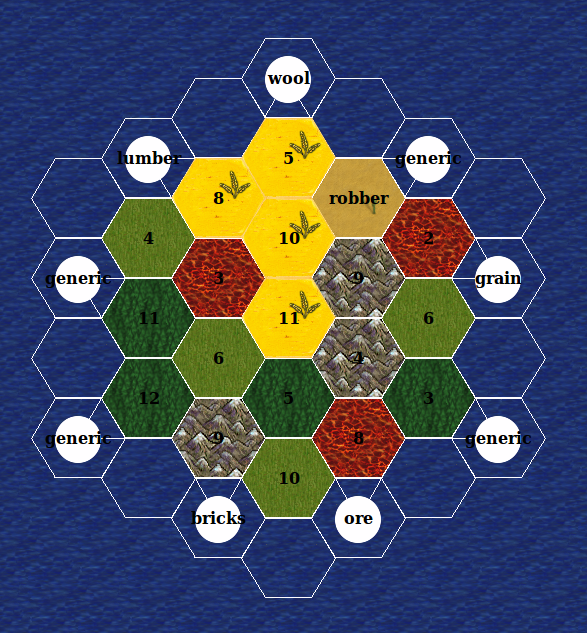
\includegraphics[width=\linewidth]{board.pdf}
  \end{center}
  \caption{Zasada numerowania sześciokątów na planszy}
  \label{board}
\end{figure}

\subsubsection{Wierzchołki}
Numerowanie wierzchołków jest nieco bardziej skomplikowanym
zadaniem. Wykorzystany został tutaj fakt, iż przy numeracji
sześciokątów przedstawionej na \imref{board}, w każdym z nich można
wyróżnić wierzchołki ,,górne'' (posiadające numer wiersza taki jak
numer wiersza sześciokąta) i ,,dolne'' (posiadające numer wiersza o
jeden większy niż numer wiersza sześciokąta). Dla ujednolicenia
schematu numeracji, konieczne stało się ponumerowanie dodatkowych
pozycji, w których nie występują wierzchołki. Omawiany sposób
numeracji został przedstawiony na \imref{nodes}. Dla planszy o
rozmiarach $x$ wierszy i $y$ kolumn, otrzymujemy tablicę wierzchołków
posiadającą wysokość $x+1$ wierszy i szerokość $2y+2$ kolumn.

\begin{figure}[ht]
  \begin{center}
    \includegraphics[width=\linewidth]{nodes.pdf}
  \end{center}
  \caption{Zasada numerowania wierzchołków na planszy}
  \label{nodes}
\end{figure}

\subsubsection{Krawędzie}
Krawędzie numerowane są na podobnej zasadzie co wierzchołki. Również
niezbędne okazało się wprowadzenie niepowiązanych z sześciokątami
pozycji. Sposób numeracji krawędzi został przedstawiony na
\imref{edges}. Plansza o rozmiarach $x$ wierszy i $y$ kolumn, posiada
tablicę krawędzi o wysokości $x+1$ wierszy i szerokości $3y+4$ kolumn.

\begin{figure}[ht]
  \begin{center}
    \includegraphics[width=\linewidth]{edges.pdf}
  \end{center}
  \caption{Zasada numerowania krawędzi na planszy}
  \label{edges}
\end{figure}

\subsubsection{}

\begin{equation}
  \begin{split}
    HEX_{adj}=
    \{
    (x-1; y+1),
    (x-1; y),
    (x; y-1),\\
    (x+1; y-1),
    (x+1; y),
    (x; y+1)
    \}
  \end{split}
  \label{hexhexes}
\end{equation}
\begin{equation}
  \begin{split}
    NODE_{adj}=\{
    (x+1; 2y),
    (x+1; 2y+1),
    (x+1; 2y+2),\\
    (x; 2y+3),
    (x; 2y+2),
    (x; 2y+1)
    \}
  \end{split}
  \label{nodehexes}
\end{equation}
\begin{equation}
  \begin{split}
    EDGE_{adj}=\{
    (x+1; 3y+2),
    (x+1; 3y+4),
    (x; 3y+6),\\
    (x; 3y+5),
    (x; 3y+4),
    (x; 3y+3)
    \}
  \end{split}
  \label{edgehexes}
\end{equation}

\begin{equation}
  HEX_{adj}=
  \left\{
    \begin{array}{l l l l}
      \begin{split}
      \{
      (x-1; \lfloor\frac{y}{2}\rfloor-1),\\
      (x-1; \lfloor\frac{y}{2}\rfloor), \\
      (x; \lfloor\frac{y}{2}\rfloor-1)
      \}
      \end{split} & \mbox{dla} & \mbox{$y=2n$,} & \mbox{$n\in\mathbb{Z}$} \\[40pt]
      \begin{split}
        \{
        (x-1; \lfloor\frac{y}{2}\rfloor), \\
        (x; \lfloor\frac{y}{2}\rfloor-1), \\
        (x; \lfloor\frac{y}{2}\rfloor)
        \}
      \end{split} & & \mbox{$y=2n+1$,} & \mbox{$n\in\mathbb{Z}$} \\
    \end{array} \right.
  \label{nodehexes}
\end{equation}
\begin{equation}
  NODE_{adj}=
  \left\{
    \begin{array}{l l}
      \{
      (x-1; 3\lfloor\frac{y}{2}\rfloor+3),
      (x; 3\lfloor\frac{y}{2}\rfloor+3),
      (x; 3\lfloor\frac{y}{2}\rfloor+2)
      \} & \mbox{dla $y=2n$, $n\in\mathbb{Z}$} \\
      \{
      (x; y+1),
      (x; y-1),
      (x+1; y-1)
      \} & \mbox{dla $y=2n+1$, $n\in\mathbb{Z}$} \\
    \end{array} \right.
  \label{nodenodes}
\end{equation}
\begin{equation}
  EDGE_{adj}=
  \left\{
    \begin{array}{l l}
      \{
      (x-1; 3\lfloor\frac{y}{2}\rfloor+3),
      (x; 3\lfloor\frac{y}{2}\rfloor+3),
      (x; 3\lfloor\frac{y}{2}\rfloor+2)
      \} & \mbox{dla $y=2n$, $n\in\mathbb{Z}$} \\
      \{
      (x; 3\lfloor\frac{y}{2}\rfloor+4),
      (x; 3\lfloor\frac{y}{2}\rfloor+2),
      (x; 3\lfloor\frac{y}{2}\rfloor+3)
      \} & \mbox{dla $y=2n+1$, $n\in\mathbb{Z}$} \\
    \end{array} \right.
  \label{nodenodes}
\end{equation}

\begin{equation}
  HEX_{adj}=
  \left\{
    \begin{array}{l l}
      \{
      (x; \lfloor\frac{y}{3}\rfloor-1),
      (x; \lfloor\frac{y}{3}\rfloor-2)
      \} & \mbox{dla $y=3n$, $n\in\mathbb{Z}$} \\
      \{
      (x-1; \lfloor\frac{y}{3}\rfloor-1),
      (x; \lfloor\frac{y}{3}\rfloor-1)
      \} & \mbox{dla $y=3n+1$, $n\in\mathbb{Z}$} \\
      \{
      (x-1; \lfloor\frac{y}{3}\rfloor),
      (x; \lfloor\frac{y}{3}\rfloor-1)
      \} & \mbox{dla $y=3n+2$, $n\in\mathbb{Z}$} \\
    \end{array} \right.
  \label{edgehexes}
\end{equation}
\begin{equation}
  NODE_{adj}=
  \left\{
    \begin{array}{l l}
      \{
      (x; 2\lfloor\frac{y}{3}\rfloor-1),
      (x+1; 2\lfloor\frac{y}{3}\rfloor-2)
      \} & \mbox{dla $y=3n$, $n\in\mathbb{Z}$} \\
      \{
      (x; 2\lfloor\frac{y}{3}\rfloor),
      (x; 2\lfloor\frac{y}{3}\rfloor-1)
      \} & \mbox{dla $y=3n+1$, $n\in\mathbb{Z}$} \\
      \{
      (x; 2\lfloor\frac{y}{3}\rfloor+1),
      (x; 2\lfloor\frac{y}{3}\rfloor)
      \} & \mbox{dla $y=3n+2$, $n\in\mathbb{Z}$} \\
    \end{array} \right.
  \label{edgenodes}
\end{equation}
\begin{equation}
  EDGE_{adj}=
  \left\{
    \begin{array}{l l}
      \begin{split}
        \{
        (x+1; y-2),
        (x+1; y-1), \\
        (x; y+1),
        (x; y-1)
        \}
      \end{split} & \mbox{dla $y=3n$, $n\in\mathbb{Z}$} \\[18pt]
      \begin{split}
        \{
        (x-1; y+2),
        (x; y-2), \\
        (x; y-1),
        (x; y+1)
        \}
      \end{split} & \mbox{dla $y=3n+1$, $n\in\mathbb{Z}$} \\[18pt]
      \begin{split}
        \{
        (x-1; y+1),
        (x; y-1), \\
        (x; y+2),
        (x; y+1)
        \}
      \end{split} & \mbox{dla $y=3n+2$, $n\in\mathbb{Z}$} \\
    \end{array} \right.
  \label{edgenodes}
\end{equation}

\begin{figure}[ht]
  \begin{center}
    \includegraphics[width=\linewidth]{erd.pdf}
  \end{center}
  \caption{Diagram związków encji}
  \label{erd}
\end{figure}

\clearpage

\bibliographystyle{plain}
\bibliography{praca}

\end{document}
